\chapter{Caso di Studio: Esempio Concreto}\label{chapter:Caso_Di_Studio}

"Collecting information is an important early step (though not the first in the intelligence cycle) To get from raw information to a finished intelligence product, researchers must process and analyze the data to determine whether it’s relevant to the investigation and turn it into actionable insights. Which is why it’s essential to lead with the question of “why is this important,” rather than focus on which tools to use." \cite{caso1}

Raccogliere informazioni è uno step fondamentale in qualsiasi operazione di intelligence, in particolare è essenziale analizzare e definire quali sono i dati rilevanti, sulla quale concentrarsi per poter effettuare trasformazioni da dati grezzi a informazioni utili.

Ottenere ciò di cui si ha bisogno dal Dark web può essere complicato, è necessario quindi aver installato un browser specializzato, come TOR. Sarà inoltre fondamentale sapere quale dominio si sta cercando (poiché come sappiamo le pagine del dark web non sono indicizzate).
Esistono tuttavia alcuni strumenti che è possibile utilizzare, (come Ahmia e Haystack), ma per la maggior parte dei casi si dovrà navigare nel dark web senza una mappa chiara.

I ricercatori OSINT trascorrono molto tempo raccogliendo informazioni da diverse piattaforme, per questo hanno ottimizzato metodologie, con le quali è possibile estrarre credenziali, nomi, domini, numeri di Whatsapp, account email Proton\footnote{\'E un servizio di posta elettronica gratuito e protetto, che utilizza la tecnologia SSL (secure socket layer) per proteggere la comunicazione tra il server e gli utenti.} ecc. 
Una volta raccolti i dati, tramite l'utilizzo dei social media e dei marketplace, sarà possibile analizzare e visualizzare le informazioni personali e tener traccia di modifiche o legami riguardo l'identità dei vari attori.

Parlando di dark web, è bene ricordare che in ambito di ricerca e raccolta dati, alcuni marketplace e forum sono specchiati sul web visibile, questo porta a numerosi vantaggi, in quanto possono offrire informazioni non visibili sul dark web, essendo spesso siti "pronti all'uso" e sviluppati con WordPress, NginX o altri CMS (Content Management System). Su questi siti specchio possono mancare restrizioni sulla privacy, possono rivelare informazioni sui server o esporre numerose informazioni.


\textbf{Parlando di sicurezza di un'organizzazione:}
Bisogna sempre essere attenti al fatto che ogni azione, anche di un singolo dipendente, può portare all'esecuzione di uno script o un malware sul sistema, compromettendo l'intera organizzazione.\\

\textbf{Trovare OSINT su un'organizzazione:}

Le aziende sono tra i soggetti più facili da cui ottenere informazioni, poiché per la loro costituzione e operatività sono tenute a presentare diverse documentazioni presso enti pubblici. Questi documenti sono spesso facilmente accessibili e consultabili, fornendo a potenziali hacker una vasta gamma di informazioni dettagliate che possono facilitare un'attività di indagine.

Effettuando una ricerca sul sito web dell'azienda o sul Registro delle Imprese (gestito dalle Camere di Commercio), è possibile ritrovare una mole di dati fondamentale per iniziare a svolgere un'attività di monitoraggio e analisi.

I siti web rappresentano una grande fonte di informazioni su un'organizzazione, sia dal punto di vista tecnico che per la sua evoluzione e/o rebranding. Per le indagini OSINT, i siti web vengono spesso analizzati per le loro informazioni tecniche, per reperire informazioni quali, chi li ha registrati, che server sono in utilizzo e da quale software vengono gestiti.
Tutte queste informazioni possono essere raccolte attraverso servizi e tools.

Infine il sito web aziendale, può mettere a disposizione un numero elevato di informazioni, per esempio file lasciati pubblici per errore o informazioni che potrebbero non essere più presenti ma essere stati parte del sito web in passato. Con strumenti come l'Internet Archive o la Wayback Machine possiamo visualizzare come si presentava un sito web e come è cambiato nel tempo, confrontandoli è possibile evidenziare cambiamenti organizzativi, nuovi collaboratori o dipendenti che non fanno più parte dell'organizzazione. 
\newpage


\begin{figure}[ht]
	\centering
	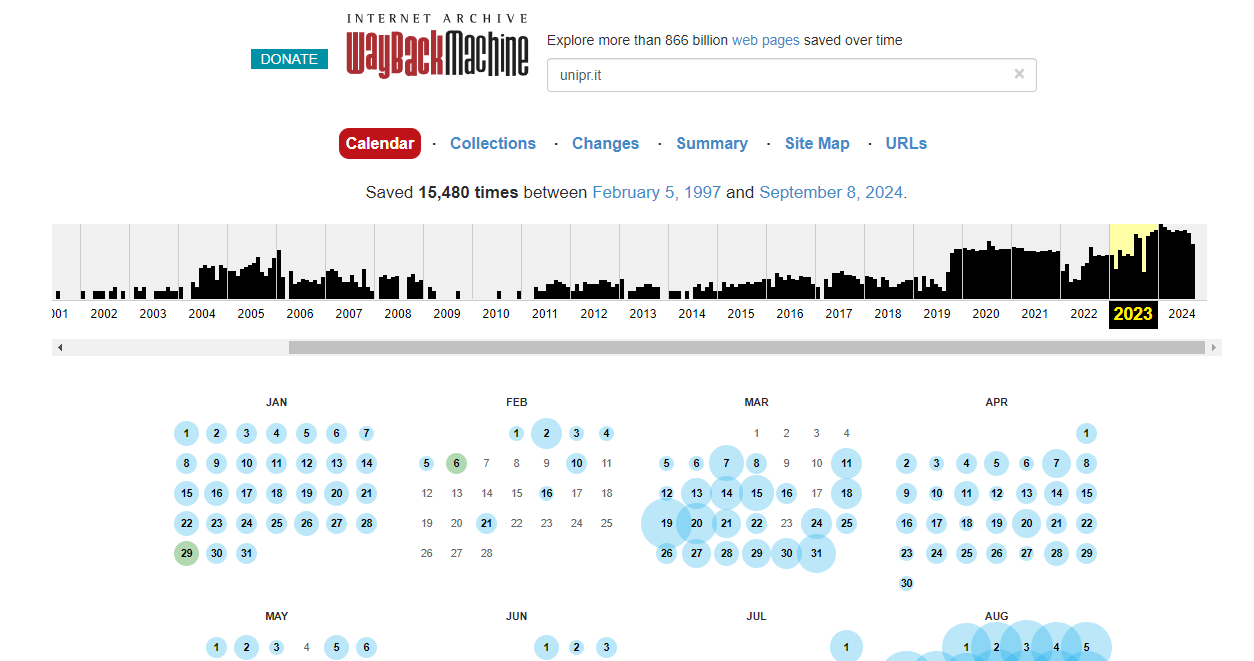
\includegraphics[width=1\textwidth]{Immagini/caso1.png}
	\caption{Wayback Machine}
	\label{fig:onecaso}
\end{figure}


Vediamo poi il "Google Dorking"\footnote{I dork sono comandi utili per affinare i risultati di una ricerca, permettendo di trovare risultati precisi} che è un'altra modalità per trovare file e altri dettagli lasciati accidentalmente pubblici su Internet. Strutturando le query di ricerca di Google, e cercando determinati tipi di pagine o file, è facile trovare componenti o informazioni all'interno del sito web che potrebbero contenere informazioni riservate.\cite{caso2}


\section{Obbiettivo}\label{sec:cap_sec_caso1}

Gli obiettivi del caso di studio sono mirati a esaminare come il Dark Web possa essere utilizzato come risorsa OSINT di un'azienda, per la protezione dei propri asset. In particolare, l'obiettivo è quello di configurare e utilizzare una serie di vulnbox, ambienti appositamente creati, configurati e isolati per condurre attività di monitoraggio e analisi.

Questi ambienti consentiranno di simulare scenari realistici di raccolta dati, protezione e prevenzione, fornendo un terreno sicuro e circoscritto per sperimentare e comprendere le procedure operative standard (SOP) per la gestione degli incidenti di sicurezza. Attraverso l'utilizzo di strumenti come Maltego, SpiderFoot, Shodan, e piattaforme di monitoraggio del dark web come DarkOwl Vision o Recorded Future, verranno eseguite attività di raccolta di informazioni, identificazione di minacce, analisi delle vulnerabilità e monitoraggio delle menzioni aziendali nel Dark Web.

È fondamentale per questo studio rilevare come sia possibile utilizzare i servizi presenti sul Dark Web per la protezione, tramite strumenti OSINT, dei dati e delle infrastrutture dell'organizzazione. Una volta identificato un attacco, verranno seguite una serie di procedure per il contenimento e la mitigazione del problema. Queste includeranno l'aggiornamento delle regole di sicurezza nei sistemi SIEM\footnote{Soluzione che consente alle organizzazioni di rilevare, analizzare e rispondere alle minacce di sicurezza prima che compromettano le operazioni aziendali.}, l'implementazione di contromisure adeguate come patching e rafforzamento delle configurazioni, e l'esecuzione di penetration testing per verificare l'efficacia delle difese.

Inoltre, sarà indispensabile implementare programmi di formazione continua per i dipendenti per aumentarne la consapevolezza sui rischi del dark web, del phishing e dell'ingegneria sociale. Infine, verrà preparato un piano di azione per il futuro, che includerà il monitoraggio continuo, la revisione periodica delle policy di sicurezza e la risposta agli incidenti per garantire la resilienza dell'organizzazione contro minacce emergenti.


\begin{figure}[ht]
	\centering
	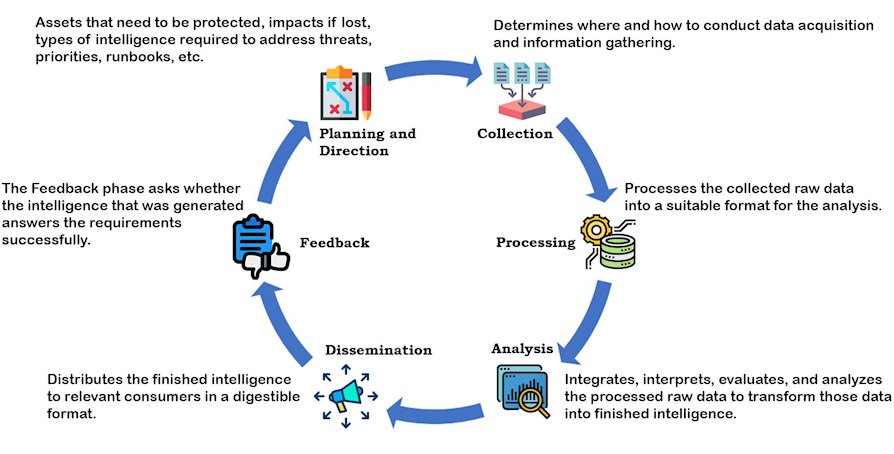
\includegraphics[width=1\textwidth]{Immagini/caso2.jpeg}
	\caption{Cyber Threat Intelligence Cycle}
	\label{fig:twocaso}
\end{figure}


Nel nostro caso concreto:

Considerando l'infrastruttura di una Startup tecnologica, impegnata nel fornire software di revenue management\footnote{RMS, è un software che aiuta le aziende a ottimizzare il volume d'affari delle attività e per la gestione delle entrate in modo rapido ed efficiente.}, utilizzando i big data e sofisticati algoritmi di intelligenza artificiale, fa previsioni precise e utili sul comportamento di prenotazione degli utenti nell'acquisto di biglietti aerei per diverse compagnie. Il software è indispensabile per effettuare previsioni e per adattare in modo rapido ed efficace le misure di comunicazione, di marketing e per adattare i prezzi al meglio.

 Con l’aiuto di un database completo, in cui confluiscono tutti i dati sul comportamento di prenotazione, e di sofisticati strumenti analitici, i programmi di Revenue Management fanno previsioni sul comportamento dei futuri clienti.

 La startup è di medie dimensioni con circa 70 dipendenti e è attiva da circa 5 anni, ha una presenza online consolidata, un'applicazione web, una mobile e un sito. 

 Questa startup può presentare vulnerabilità riguardanti il sito web principale (dedicata a clienti e partner), tramite i servizi di posta elettronica aziendale, tramite i dati sensibili dei clienti e i dati proprietari (codice sorgente ecc.).

 Come vedremo subirà un attacco in cui le credenziali di accesso di dipendenti e amministratori di sistema verranno sottratte, e successivamente pubblicizzate su un forum presente sul Dark Web. Con lo scopo di avere un punto d'appoggio all'interno dei sistemi aziendali (per potersi appropriare del codice sorgente, di informazioni proprietarie ecc.), e di guadagnare ricattando l'organizzazione, criptando i dati aziendali e dei clienti con un attacco di tipo Ransomware, paralizzando così le operazioni.

 Quest'attacco sarà il risultato di un incidente di sicurezza, causata da una email di phising e diverse tattica di social engineering\footnote{O ingegneria sociale è una tecnica di cyber attack basata sullo studio del comportamento delle persone col fine di manipolarle e appropriarsi di informazioni confidenziali}. Gli analisti della startup utilizzeranno strumenti OSINT per monitorare forum di hacker e marketplace sul dark web, per cercare menzioni relative alla startup e dei suoi asset.
Durante il monitoraggio, verrà rilevato un post su un forum di hacker dove un utente anonimo sta tentando di vendere credenziali rubate appartenenti ai dipendenti della startup.

Utilizzando strumenti di monitoraggio del dark web verranno raccolti dati e menzioni relative alla startup e verranno ricercate le connessioni tra l'attore malevolo e l'organizzazione.

Infine verranno fornite checklist per l'implementazione delle contromisure, configurati Sistemi di Monitoraggio Continui (ad esempio sistemi SIEM), verranno avviati programmi di formazione per l'organizzazione sui rischi del social engineering e del phishing, e verranno eseguiti regolarmente test di penetration testing.


\newpage
\section{Preparazione dell'Ambiente di Lavoro}\label{sec:cap_sec_caso2}

\begin{figure}[ht]
	\centering
	\includegraphics[width=1\textwidth]{Immagini/infrastruttura.png}
	\caption{Infrastruttura ricreate in ambiente sandbox}
	\label{fig:threecaso}
\end{figure}

Il sistema sarà formato da una macchina principale sotto la quale avremo l'integrazione di 3 ambienti.\\

Nello specifico tre macchine virtuali (o server) per le diverse funzioni\footnote{Opens Source Intelligence, Pentesting e SIEM (Security Information and Event Management)}, tutte collegate a un Main PC che opera da host. 
\'E implementato l'uso di un firewall per proteggere il traffico di rete, per prevenire accessi non autorizzati e per monitorare il traffico in entrata e uscita.
\'E implementato inoltre l'isolamento delle macchine virtuali per circoscrivere ciascuna funzione (monitoraggio, pentesting, Gestione degli eventi), per la sicurezza e per limitare i danni in caso di compromissione di una delle macchine.

\begin{enumerate}
    \item \textbf{Macchina OSINT/Dark Web Monitoring:} 
    Una macchina virtuale Linux (Con OS Ubuntu) configurata con strumenti per la raccolta di informazioni e navigazione sicura nel dark web.
    Questa macchina è utilizzata per raccogliere informazioni di intelligence e monitorare le attività nel dark web relative all'organizzazione.
    Con installati strumenti quali Maltego, SpiderFoot, Shodan.
    Sarà utilizzata per la raccolta automatizzata di informazioni da fonti pubbliche, dal dark web, per la scansione di servizi esposti e la raccolta di informazioni sulle vulnerabilità conosciute.
    \item \textbf{Macchina SIEM e Log Management:}
     Un server dedicato con Elastic Stack o Splunk, configurato per raccogliere, analizzare e visualizzare i log di rete e di sistema. Su questa macchina verranno eseguite simulazioni di attacco (es. penetration testing) per identificare e verificare le vulnerabilità nelle risorse esposte dell'organizzazione e per raccogliere log da varie fonti e visualizzare gli eventi in dashboard interattive secondo regole di correlazione.
    \item \textbf{Macchina di Pentesting:}
    \'E una macchina virtuale con Kali Linux dedicata alle attività di penetration testing. Esegue simulazioni di diversi attacchi per identificare e verificare le vulnerabilità esposte dell'organizzazione.
    Utilizzando strumenti come Metasploit, Nmap, Burp Suite per testare le infrastrutture e le reti.
\end{enumerate}



L'analisi dei dati si concentrerà sul Flusso di Informazioni OSINT e Dark Web verso i SIEM e il Log Management:\\

La macchina \textbf{OSINT/Dark Web Monitoring} raccoglie sia le informazioni pubbliche che quelle nel dark web relative all'organizzazione, come per esempio potenziali compromissioni, menzioni su forum di hacker, e credenziali esposte. I risultati pertinenti\footnote{indicatori di compromissione, indirizzi IP sospetti, Hash e domini malevoli} vengono inviati alla macchina SIEM e Log che creerà regole di correlazione e avvisi di sicurezza.
Una volta analizzati, nel caso in cui venisse rilevata un'anomalia, credenziali compromesse o altri tipi di threat, il SIEM può essere configurato per monitorare l'utilizzo di quelle informazioni all'interno della rete e generare avvisi nel caso in cui venissero utilizzate.

Nel caso in cui il \textbf{SIEM e Log Management} identifichino attività sospette o vulnerabilità segnalate anche dagli avvisi, queste vengono trasmesse alla macchina di Pentesting, dove i penetration tester possono concentrarsi sulle aree identificate e segnalate come vulnerabili.
Per esempio se il SIEM rileva traffico sospetto su una porta aperta, il team di pentesting può utilizzare strumenti come Nmap e Metasploit per testare ulteriormente quella specifica area, questi test mirati di attacchi brute force o exploit, serviranno per verificare l'efficacia delle misure di sicurezza impostate.

Alla fine i risultati ottenuti saranno utilizzati per aggiornare le regole di sicurezza del SIEM, per assicurare che futuri tentativi di attacco possano essere identificati e mitigati il prima possibile.
In aggiunta le nuove minacce o exploit identificate, durante le attività di pentesting, possono suggerire la necessità di un'investigazione più approfondita delle informazioni OSINT e nel monitoring del Dark Web, in modo da prevenire potenziali exploit e attacchi zero-day\footnote{Descrive vulnerabilità scoperte recentemente e utilizzate da hacker. Il termine "zero-day" si riferisce al fatto che il fornitore o lo sviluppatore è appena venuto a conoscenza della falla e quindi ha "zero giorni" di tempo per correggere l'anomalia}.


\section{Raccolta di Dati tramite OSINT}\label{sec:cap_sec_caso3}

Vediamo di seguito la raccolta e l'analisi di alcuni dati utilizzando il server di OSINT e Dark Web Monitoring, collegandoci alla macchina virtuale creata con Oracle VM VirtualBox, è possibile avviare il primo strumento con la quale andremo a verificare la possibile presenza di dati riguardanti la nostra azienda sul dark web.

Per prima cosa andremo ad installare il browser TOR e a collegarci a una VPN.

\tcbset{
    frame code={},
    center title,
    left=0pt,
    right=0pt,
    top=0pt,
    bottom=0pt,
    colback=gray!70,
    colframe=white,
    width=\dimexpr\textwidth\relax,
    enlarge left by=0mm,
    boxsep=4pt,
    arc=0pt,outer arc=0pt,
    }
    \begin{tcolorbox}
\textsc{sudo apt install -y tor torbrowser-launcher}
    \end{tcolorbox}

Registrare e successivamente eseguire tramite il terminale il nostro browser, posizionandosi sulla location delle cartelle di installazione:

    \begin{tcolorbox}
\textsc{./start-tor-browser.desktop --register.app}
    \end{tcolorbox}

Possiamo poi collegarci e creare un account su Darkowl.

\begin{figure}[ht]
	\centering
	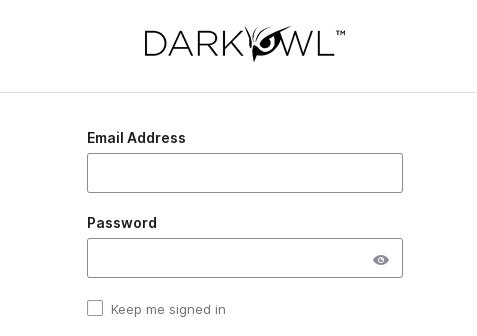
\includegraphics[width=0.4\textwidth]{Immagini/caso4.png}
	\caption{Login di Darkowl}
	\label{fig:fourcaso}
\end{figure}

Una volta create le credenziali di accesso, sarà possibile effettuare una ricerca con Darkowl Vision: Ci colleghiamo tramite il sito web, dove ci si presenta una barra di ricerca, con la quale potremo fare una ricerca sul nome dell'organizzazione, sul dominio o su qualsiasi dato che ci può interessare.

\begin{figure}[ht]
	\centering
	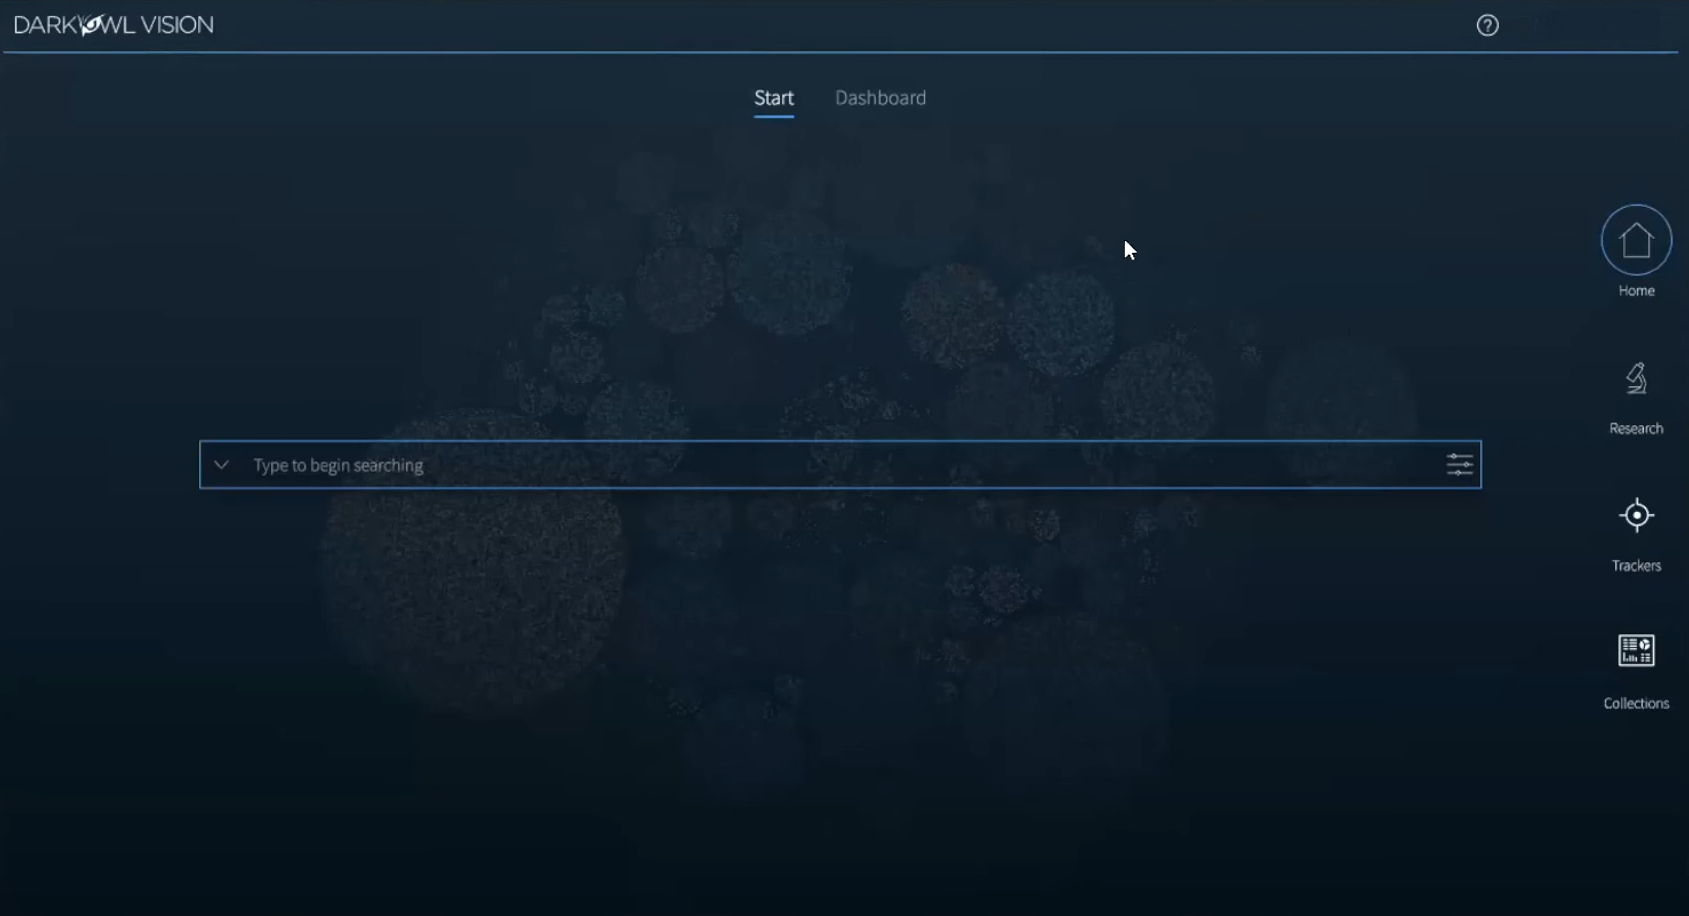
\includegraphics[width=0.8\textwidth]{Immagini/caso5.png}
	\caption{Landing page Darkowl}
	\label{fig:fivecaso}
\end{figure}

Andiamo a fare una ricerca utilizzando la keywork "wordpress.com", questo andrà a cercare sul dark web ogni menzione o dato presente (visitando forum, siti web, conversazioni ecc.) riguardano l'oggetto della ricerca:

\begin{figure}[h]
	\centering
	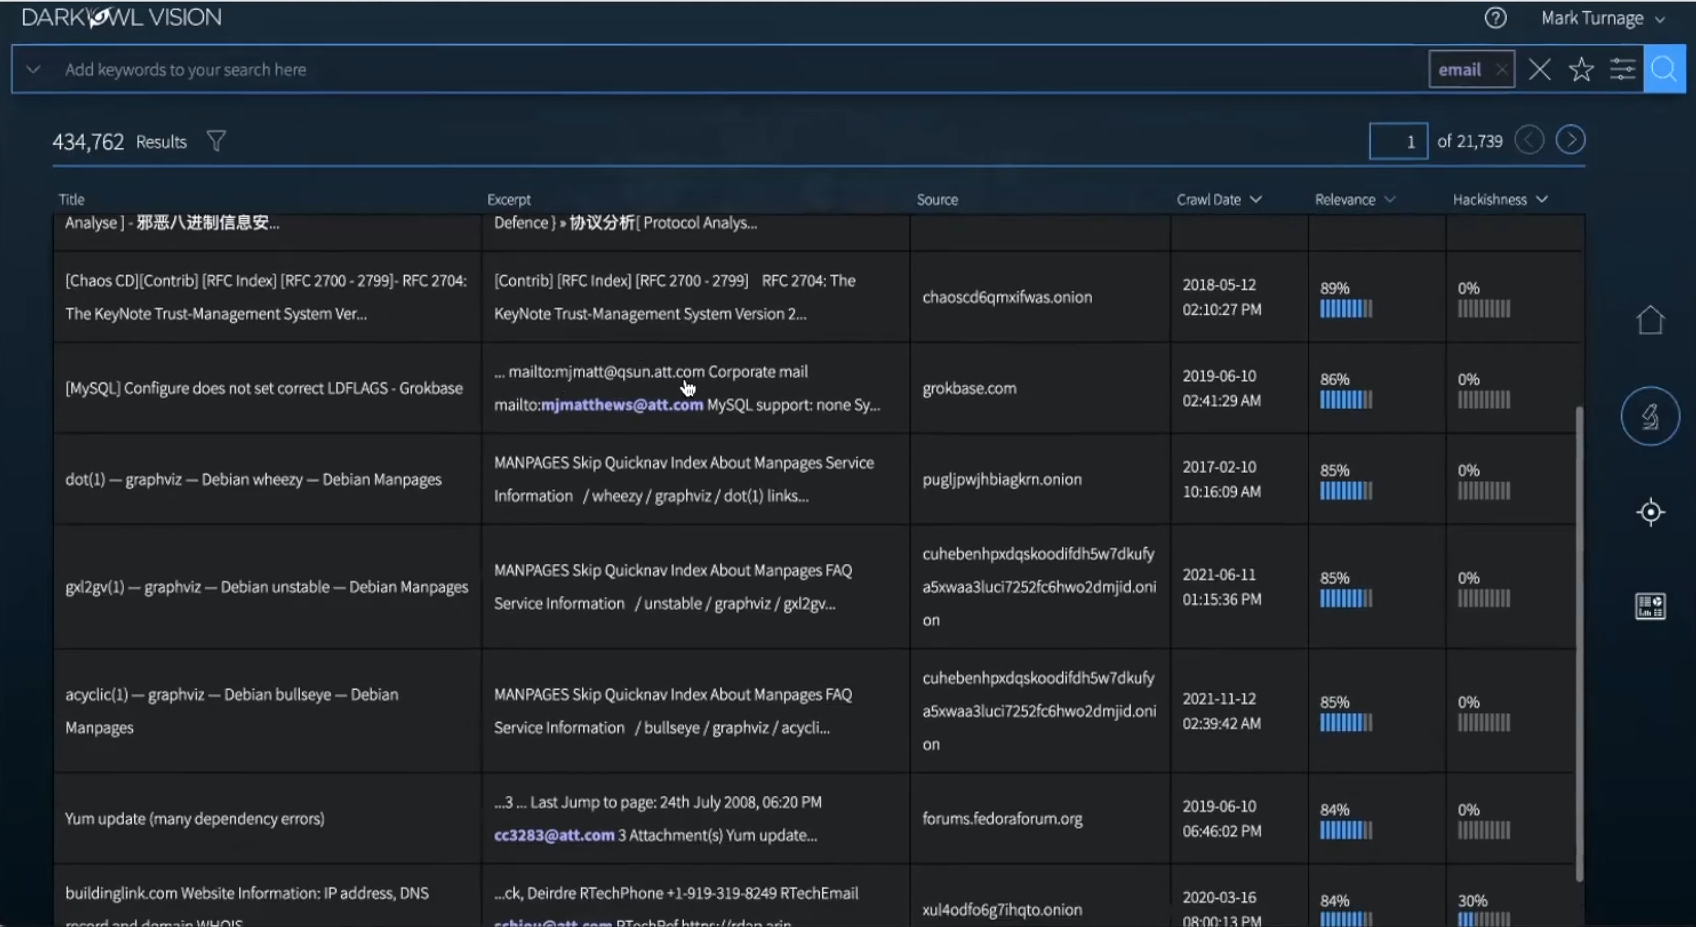
\includegraphics[width=0.8\textwidth]{Immagini/caso6.png}
	\caption{Risultato di una possibile ricerca}
	\label{fig:sixcaso}
\end{figure}

In questo caso possiamo vedere circa 434 mila risultati e navigando il sito osserviamo una serie di risultati, che possono essere email, credenziali o altre tipologie di informazione.
I dati possono essere presentati in tanti modi differenti e organizzati/riordinati per data, nome o importanza.

Vedremo per esempio un timestap con il periodo di estrazione del dato dal dark web e sarà possibile ordinarli per rilevanza e "hackishness"\footnote{Indica quanto è rilevante e pericoloso quel determinato risultato}, questo indicatore sarà molto elevato nel caso in cui il risultato contenesse informazioni sensibili o possibili password in chiaro.

\begin{figure}[ht]
	\centering
	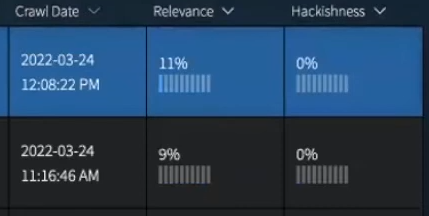
\includegraphics[width=0.5\textwidth]{Immagini/caso7.png}
	\caption{Rilevanza dell'output e hackishness}
	\label{fig:sevencaso}
\end{figure}

Come abbiamo visto, questo è uno strumento diretto e intuitivo, soprattutto per un team alla ricerca di informazioni specifiche o un possibile hacker alla ricerca di informazioni in chiaro sul darkweb.\\

Successivamente alla raccolta dei dati con l'utilizzo di uno strumento di data mining e organizzazione delle informazioni, per esempio maltego sarà possibile andare a identificare e visualizzare relazioni tra diverse informazioni o dati.

Prima di eseguire il programma sarà indispensabile installare una versione di java sul sistema operativo:

\begin{figure}[ht]
	\centering
	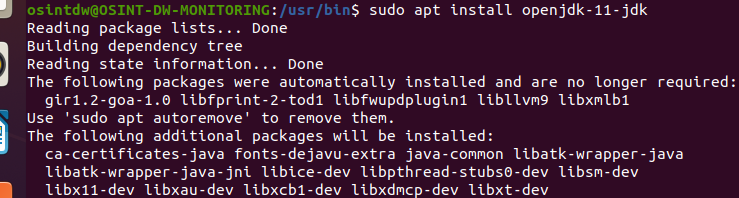
\includegraphics[width=0.8\textwidth]{Immagini/caso9.png}
	\caption{Installazione di Java}
	\label{fig:eightcaso}
\end{figure}

Terminato il download e l'installazione sarà possibile eseguire il programma e creare un nuovo mappatura (successivamente alla creazione di un account sul sito ufficiale).
Una volta selezionato il web browser ci verrà chiesto di scegliere tutti o una serie di transforms:

\begin{figure}[ht]
	\centering
	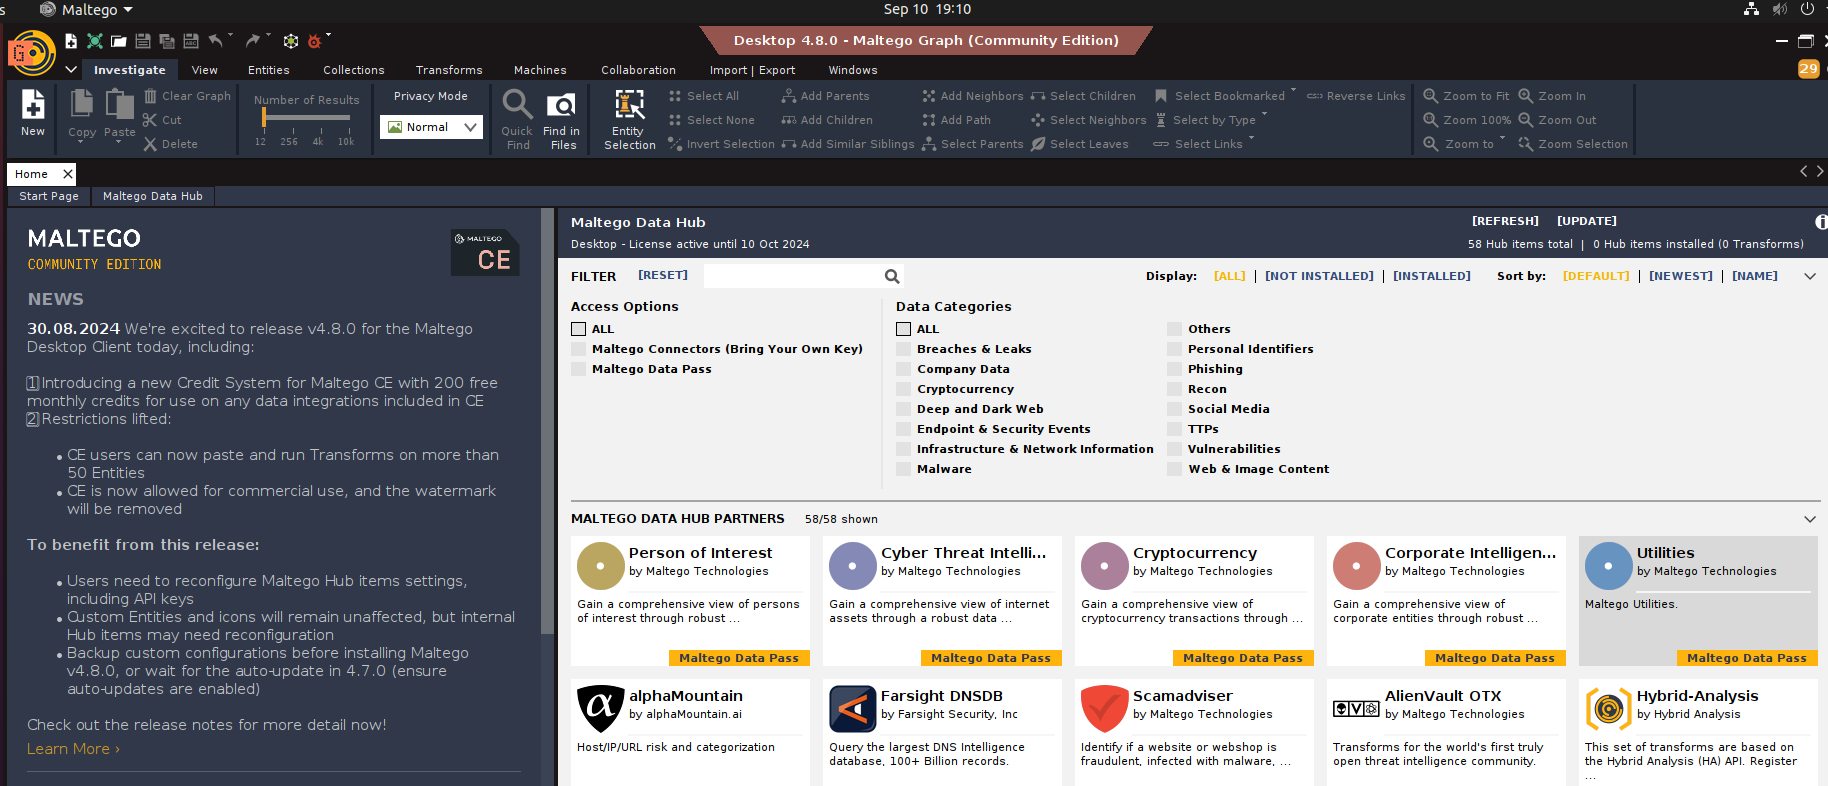
\includegraphics[width=0.8\textwidth]{Immagini/caso10.png}
	\caption{Transforms in Maltego}
	\label{fig:ninecaso}
\end{figure}

Scelti i trasform e il relativo API (per esempio filtrando solo per "Breaches e leaks, dark web e phising" troveremo i seguenti API con la quale andare a creare le nostre ricerche:

\begin{figure}[ht]
	\centering
	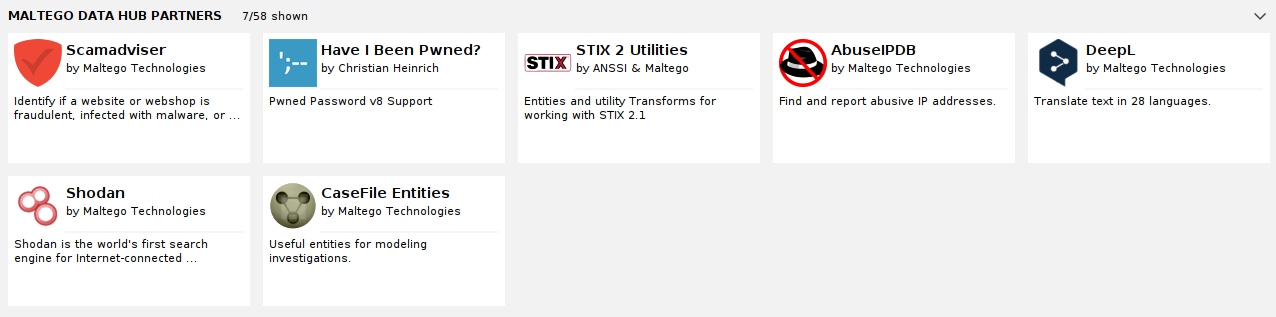
\includegraphics[width=0.8\textwidth]{Immagini/caso11.png}
	\caption{Transforms da utilizzare nel caso di una ricerca OSINT-Dark Web}
	\label{fig:tenecaso}
\end{figure}

Maltego mette a disposizione tantissimi tool e API che una volta installati, ci permetterà di creare una mappatura dei nostri dati, facendo una ricerca sui dati che abbiamo recuperato in precedenza o dati correlati.

Ricercando una serie di entità e inserendo dati di cui siamo a conoscenza o chiedendo a Maltego (con l'utilizzo delle API installate) di recuperare informazioni (dal clear web e soprattutto dal dark web) sul target potremo andare a creare il nostro dataset formato da informazioni, quali:

\begin{enumerate}
    \item Persone
    \item Organizzazioni
    \item Siti Web
    \item Indirizzi IPV4
    \item Indirizzi cryto
    \item Canali social
\end{enumerate}

La mappatura risulterà quindi una serie di dati e i collegamenti che siamo in grado di recuperare su di essi:

\begin{figure}[ht]
	\centering
	
\includegraphics[width=0.8\textwidth]{Immagini/caso12.png}
	\caption{Mappatura di esempio, dati universitari ed email personale}
	\label{fig:elevencaso}
\end{figure}

Da sottolineare che questo tipo di investigazione può essere rivolto a qualsiasi individuo, organizzazione o professionista.

\section{Analisi delle Informazioni dal Dark Web}\label{sec:cap_sec_caso4}

Una volta terminato il mapping dei dati e recuperate tutte le informazioni comprese le loro origini, saremo in grado di seguire una serie di steps per mitigare i rischi di ulteriori compromissioni e saremo in grado di rafforzare la sicurezza della nostra organizzazione, per evitare ulteriori data breaches. 

Verrà utilizzata la seconda macchina creata "SIEM E LOG MANAGMENT" per eseguire analisi forensi, verificando come detto sopra i relativi log di sistema.

Utilizzeremo Splunk per tracciare gli eventi sulla macchina e possibili falle di sistema, e andando con questi dati ad alimentare l'input dei dati con informazioni locali.

\begin{figure}[H]
	\centering
	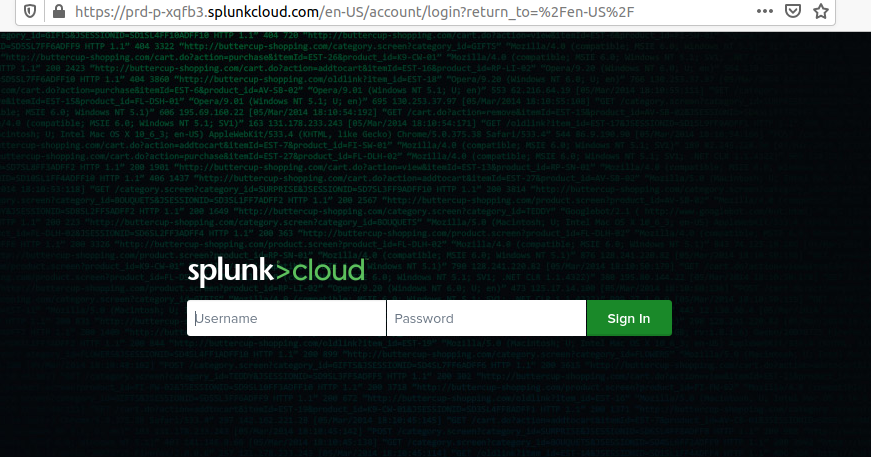
\includegraphics[width=0.8\textwidth]{Immagini/caso13.png}
	\caption{Landing page Splunk}
	\label{fig:twelvecaso}
\end{figure}

\begin{figure}[H]
	\centering
	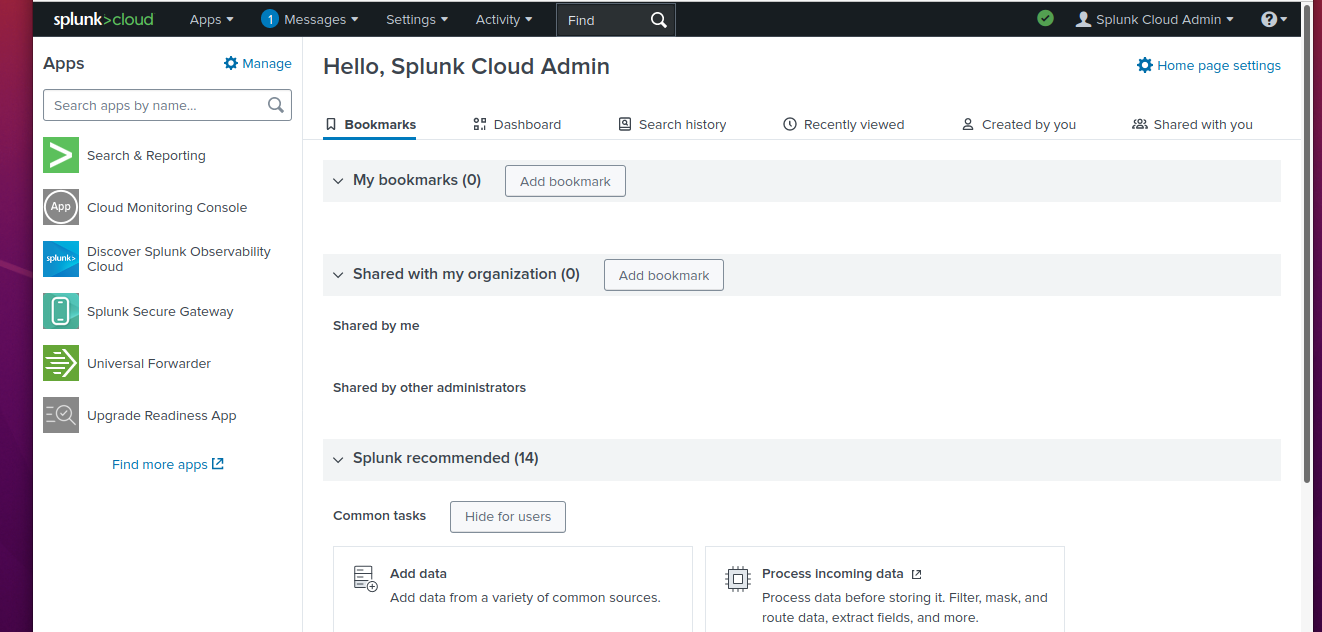
\includegraphics[width=0.8\textwidth]{Immagini/caso14.png}
	\caption{Homepage Splunk}
	\label{fig:therteencaso}
\end{figure}

Andremo ad eseguire la verifica di alcune attività in locale\footnote{Da ricordare che come ogni tool di monitoring è illegale eseguire scansioni su macchine di cui non si è proprietari o per le cui non si ha un'autorizzazione}.

Imposteremo i dati che vogliamo vengano analizzati (Local event log collection) e imposteremo la tipologia di dati in questo caso:

\begin{enumerate}
    \item Applications
    \item Security
    \item System
\end{enumerate}

Nella barra di ricerca andremo ad inserire il carattere speciale "*" con la quale andremo a recuperare ogni tipo di evento sul sistema.
E in basso verrà visualizzato il risultato. 

\begin{figure}[ht]
	\centering
	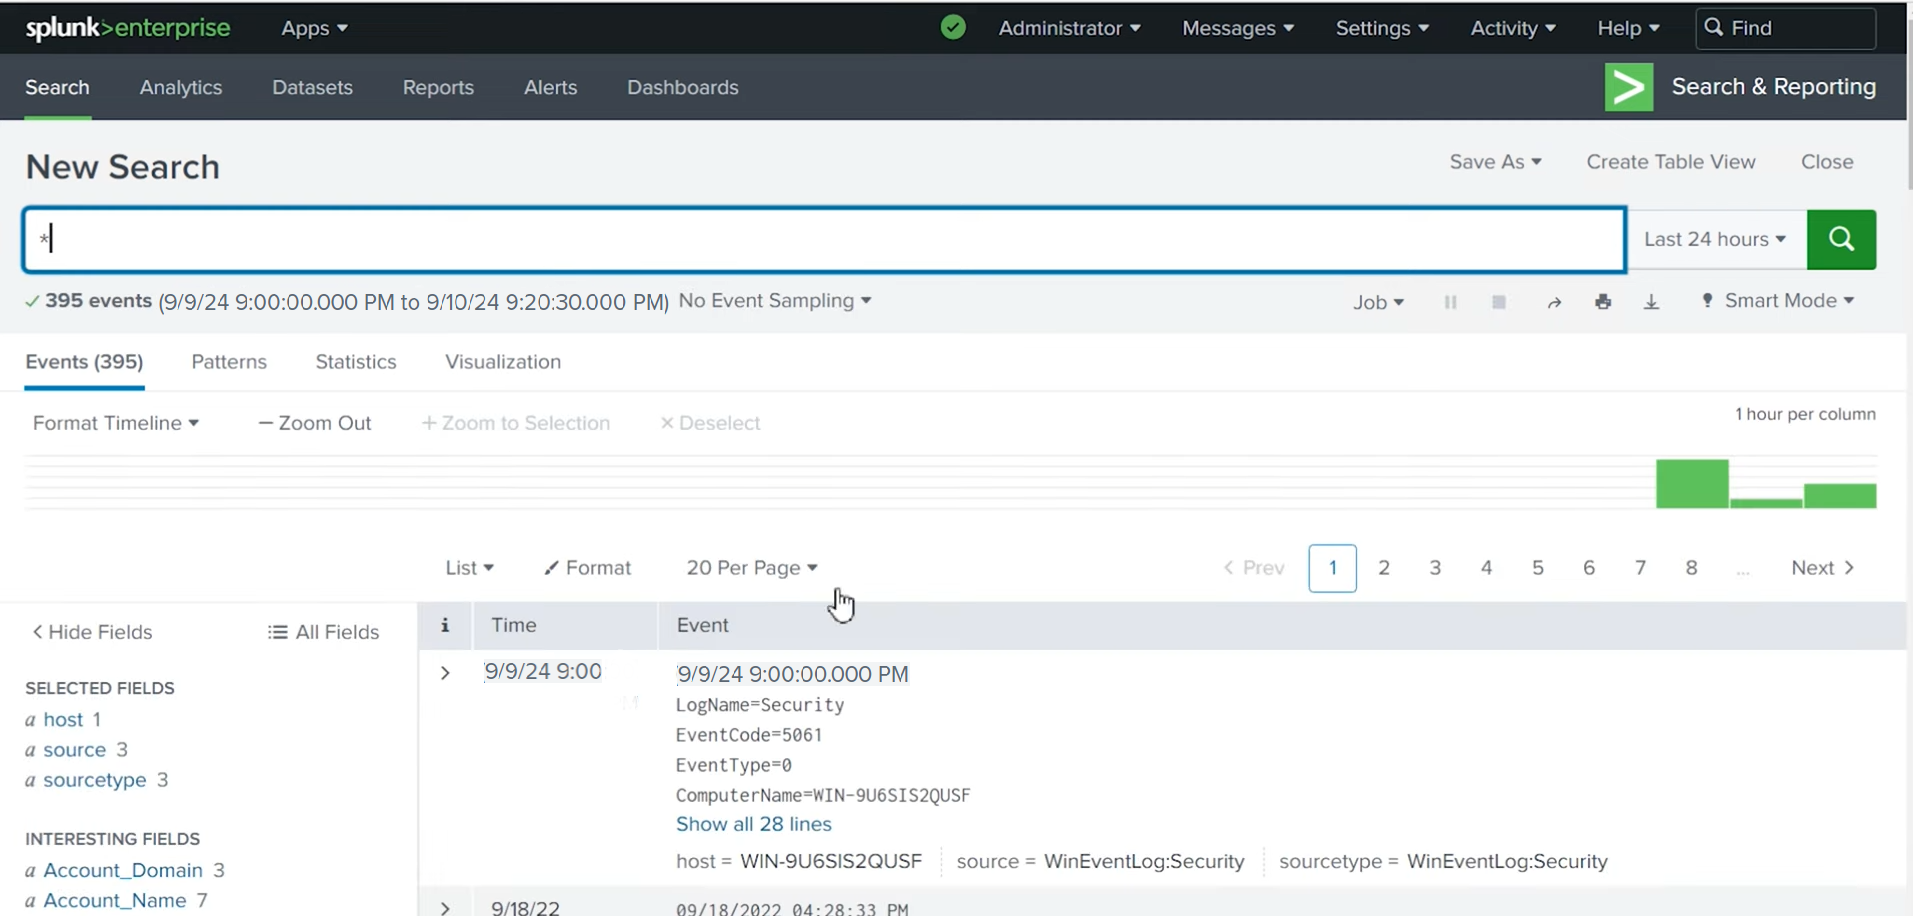
\includegraphics[width=0.8\textwidth]{Immagini/caso15.png}
	\caption{Ricerca generale di eventi}
	\label{fig:fourteencaso}
\end{figure}

Sarà in oltre possibile fare ricerche specifiche per un host come in questo caso e osservare ogni azione/attività che viene eseguita.
Filtrare per la sorgente e eventualmente il codice dell'evento.\\

Per rendere la visualizzazione ancora più chiara e semplice, i dati raccolti potranno essere rappresentati all'interno di dashboards.

Il passo successivo dell'investigazione e della protezione dei dati avrà come obbiettivo il contenimento e l'isolamento dei dati.

Identificando i sistemi compromessi o a rischio e isolando immediatamente questi asset dalla rete aziendale per prevenire ulteriori accessi non autorizzati.
Con l'utilizzo di regole sul firewall e sistemi IDS/IPS\footnote{Sistemi di rilevamento e prevenzioni delle intrusioni} per bloccare le comunicazioni con gli IP o i domini associati ad attività sospette.\\

Un altro step utile sarà quello di richiedere un reset obbligatorio delle credenziali per tutti gli utenti coinvolti (in particolare se sono state rilevate credenziali compromesse).
Invalidare tutti i token di sessione attivi e forza una ri-autenticazione su tutti i sistemi critici.\\

Una volta che il sistema sarà tornato in sicurezza, si passerà alla fase di verifica e test dei sistemi, utilizzando la VM di Penetration Testing, e con l'utilizzo del software Metasploit andremo a verificare che i sistemi siamo aggiornati e patchati con le ultime realese di sicurezza. \\

Collegandoci alla CLI di Metasploit avremo la possibilità di testare numerosi exploit sulle nostre macchine.
Una volta che avremo raccolto tutti i dati necessari attraverso la macchina di Penetration testing, agiremo come segue:

Avvieremo il programma:

\tcbset{
    frame code={},
    center title,
    left=0pt,
    right=0pt,
    top=0pt,
    bottom=0pt,
    colback=gray!70,
    colframe=white,
    width=\dimexpr\textwidth\relax,
    enlarge left by=0mm,
    boxsep=4pt,
    arc=0pt,outer arc=0pt,
    }
    \begin{tcolorbox}
\textsc{sudo msfconsole}
    \end{tcolorbox}

\begin{figure}[ht]
	\centering
	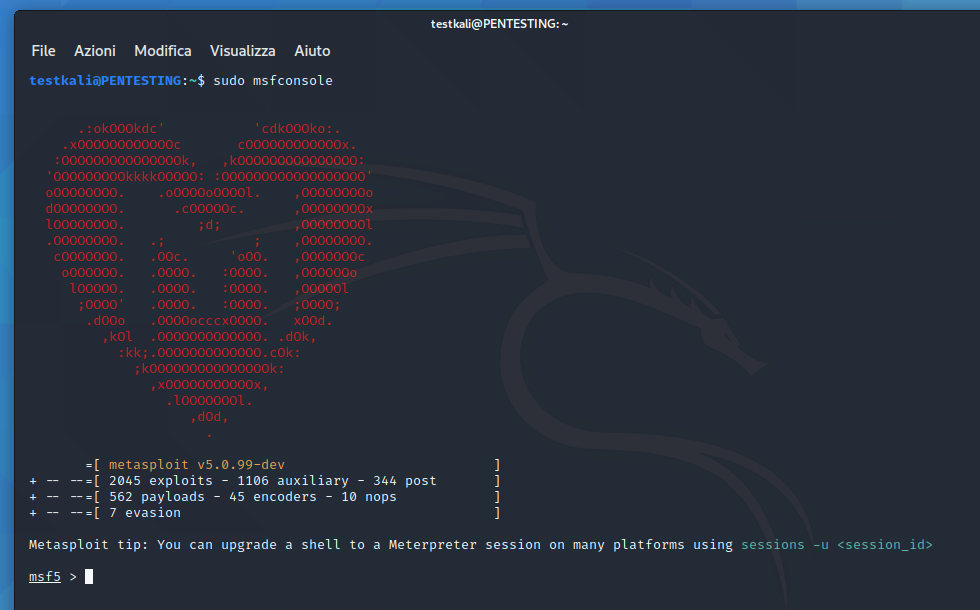
\includegraphics[width=0.8\textwidth]{Immagini/caso16.png}
	\caption{Metasploit}
	\label{fig:fiftheencaso}
\end{figure}

Una volta collegati, potremo cercare una serie di comandi che il software mette a disposizione e con il comando seguente andremo a filtrare solo i moduli che contengono "scanner":

    \begin{tcolorbox}
\textsc{grep scanner search smb}
    \end{tcolorbox}

\begin{figure}[ht]
	\centering
	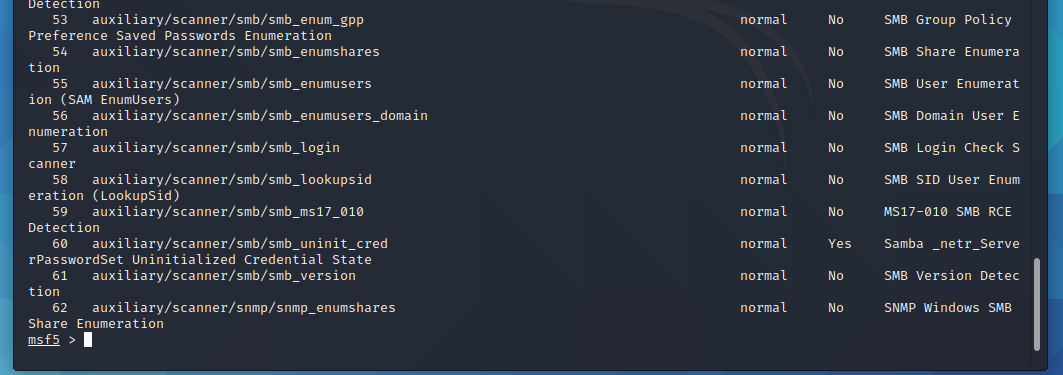
\includegraphics[width=0.8\textwidth]{Immagini/caso17.png}
	\caption{Ricerca di attacchi di tipo smb}
	\label{fig:sixtheencaso}
\end{figure}

Andremo ad eseguire un comando in particolare che fino a pochi anni fa, fu uno dei maggiori exploit e la causa di diversi attacchi di tipo Ransomware (veniva usato questo specifico comando di exploit per ottenere accesso alle macchine delle vittime e poter eseguire gli attacchi):

    \begin{tcolorbox}
\textsc{use auxiliary/scanner/smb/smb\_ms17\_010}
    \end{tcolorbox}

Andremo poi a selezionare le opzioni e con \textbf{RHSOTS}, la macchina bersaglio. Una volta eseguito l'attacco però, riscontriamo nel nostro caso che il sistema non è suscettibile a questa tipologia di exploit.

\begin{figure}[ht]
	\centering
	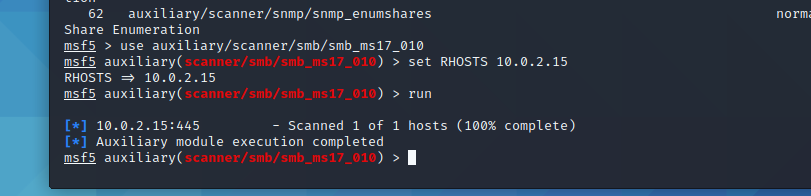
\includegraphics[width=0.8\textwidth]{Immagini/caso18.png}
	\caption{Vulnerabilità Non Rilevata}
	\label{fig:seventheencaso}
\end{figure}

Nel caso in cui lo fosse stato, la risposta che avremmo ricevuto sarebbe stata la seguente:

\begin{figure}[ht]
	\centering
	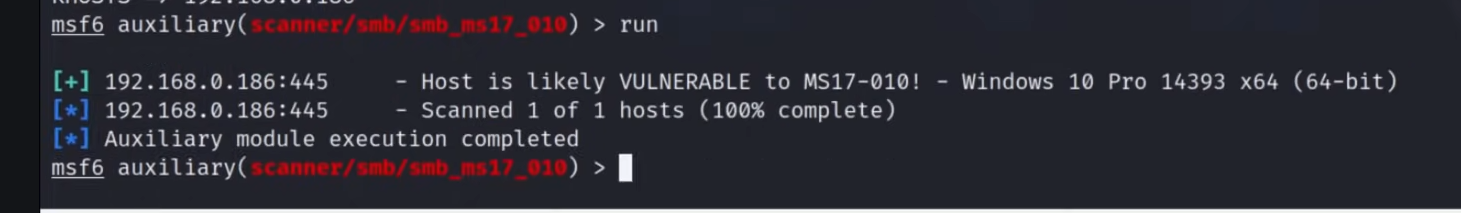
\includegraphics[width=0.8\textwidth]{Immagini/caso19.png}
	\caption{Vulnerabilità Rilevata}
	\label{fig:eightheencaso}
\end{figure}

In questa casistica sarebbe poi stato possibile accedere alla macchina e avanzare con l'attacco.
Questa vulnerabilità, una volta rilevata, sarebbe quindi da correggere immediatamente.\\


Verificate le varie vulnerabilità, l'obbiettivo diventa quello di configura la macchina SIEM e Log Management per monitorare continuamente i log di accesso, informazioni dal dark web, gli eventi di sicurezza e le attività anomale (come questi attacchi) in tempo reale.

E quello di concentrarsi sull'educazione e sulla formazione dei dipendenti, che come abbiamo visto sono spesso l'anello più debole di un sistema di sicurezza aziendale.

Sarebbe poi indispensabile:

\begin{enumerate}
    \item Condurre sessioni di formazione continua sulla consapevolezza della sicurezza informatica, inclusi phishing, social engineering, e gestione sicura delle informazioni.
    \item Creare e distribuire SOPs (Standard Operating Procedures) per la risposta rapida agli incidenti e la gestione delle emergenze di sicurezza.
    \item Validare le Contromisure Attraverso Test di Penetration regolari.
    \item Organizzare simulazioni regolari di incidenti di sicurezza per verificare l'efficacia dei piani di risposta agli incidenti e la prontezza dei team.
    \item Integrare le informazioni raccolte dal monitoraggio del dark web nel ciclo di sviluppo della sicurezza aziendale, migliorando continuamente le difese in base alle nuove minacce e ai trend osservati.
\end{enumerate}


\section{Risultati}\label{sec:cap_sec_caso5}

Vediamo quindi come con il caso di studio appena proposto, il Dark Web venga utilizzata come risorsa di Open Source Intelligence per proteggere gli asset di un'organizzazione, tramite la configurazione e l'utilizzo di ambienti isolati (vulnbox) e strumenti di monitoraggio. Vediamo come la nostra startup tecnologica, operante nel campo del revenue management per compagnie aeree, abbia subito un attacco di phishing che ha portato alla compromissione delle credenziali dei dipendenti (e alla loro possibile vendita su forum del Dark Web) e come tramite gli strumenti a nostra disposizione sia stato possibile analizzare il problema, impostare correzioni o come sarebbe stato possibile prevenirlo.

L'ambiente è stato creato utilizzando una combinazione di macchine virtuali, che hanno simulato i sistemi dell'organizzazione. Queste macchine includevano:

\begin{enumerate}
    \item Una macchina OSINT/Dark Web Monitoring per la raccolta di informazioni nel dark web.
    \item Una macchina SIEM e Log Management per la gestione e l'analisi dei log di sistema.
    \item Una macchina di Pentesting per simulare attacchi ed eseguire penetration testing.
\end{enumerate}

L'isolamento di queste macchine ha garantito che le attività eseguite, avvenissero in un ambiente sicuro, minimizzando i rischi in caso di compromissione.

Per il monitoraggio e la raccolta di dati tramite OSINT, abbiamo analizzato come l'utilizzo di strumenti come TOR, Maltego, SpiderFoot e piattaforme di monitoraggio come DarkOwl Vision siano indispensabili per raccogliere informazioni sensibili nel dark web riguardanti l'organizzazione.
È stato rilevato un post su un forum di hacker in cui venivano vendute credenziali rubate dei dipendenti della startup, indicando una potenziale compromissione dei sistemi aziendali.\\

Abbiamo analizzato le informazioni raccolte dal dark web e tramite strumenti di monitoraggio del dark web sono stati analizzati e identificate possibili connessioni tra l'attore malevolo e l'organizzazione.
Gli strumenti di gestione dei log, come Splunk, sono stati poi utilizzati per monitorare attività sospette, creare regole di correlazione e avvisi di sicurezza per migliorare la capacità di rilevamento e risposta dell'organizzazione.\\

Sono state introdotte contromisure per l'identificazione delle credenziali compromesse, sono state implementate contromisure come l'aggiornamento delle regole di sicurezza dei sistemi SIEM, l'applicazione di patch e il rafforzamento delle configurazioni di sicurezza.
Sono stati avviati programmi di formazione continua per i dipendenti per aumentarne la consapevolezza sui rischi del dark web, del phishing e dell'ingegneria sociale.
Sono stati implementati test regolari di penetration testing per verificare l'efficacia delle difese contro le minacce emergenti.\\

E si è evidenziata la necessità per il futuro di monitorare continuamente il dark web e le varie fonti OSINT per prevenire attacchi, di migliorare il piano di risposta agli incidenti, effettuando revisioni periodiche delle policy di sicurezza e continuare a rafforzare la resilienza dell'organizzazione contro minacce zero-day e minacce più sofisticate.